\documentclass[a4paper, 12pt]{article}

\usepackage[T2A]{fontenc}
\usepackage[utf8]{inputenc}
\usepackage[english, russian]{babel}
\usepackage[top=2cm, bottom=2cm, right=2cm, left=2cm]{geometry}
\usepackage{amsmath}
\usepackage[utf8]{inputenc}
\usepackage{graphicx}
\usepackage{subcaption}
\usepackage{float}
\usepackage{tabularx}
\usepackage{tabu}
\newcommand\tline[2]{$\underset{\text{#1}}{\text{\underline{\hspace{#2}}}}$}
\usepackage{indentfirst}
\usepackage{setspace} 
% одинарный интервал 
\singlespacing 
% полуторный интервал 
\onehalfspacing 
% двойной интервал 
\doublespacing 
% произвольный интервал 
\setstretch{1}
\usepackage{amsmath,booktabs}
\usepackage{array}
\graphicspath{ {images/} }
\usepackage{caption}
\captionsetup[figure]{name = Рисунок, labelsep = endash}
\captionsetup[table]{name = Таблица, labelsep = endash, justification=raggedright, singlelinecheck=false}
\captionsetup[table]{labelformat=simple, labelsep = endash, justification = raggedright, singlelinecheck = off, width = 0.92\textwidth} 
\begin{document} 
	\parindent=1.27cm
	\begin{titlepage}
		\centering
		{\fontsize{12pt}{5cm}\selectfont \bfseries Министерство образования и науки Российской Федерации} \\ \vspace{0.5cm}
		{\fontsize{7pt}{5cm}\selectfont ФЕДЕРАЛЬНОЕ ГОСУДАРСТВЕННОЕ АВТОНОМНОЕ ОБРАЗОВАТЕЛЬНОЕ УЧРЕЖДЕНИЕ ВЫСШЕГО ПРОФЕССИОНАЛЬНОГО ОБРАЗОВАНИЯ} \\ 
		\vspace{1cm}
		{\fontsize{12pt}{5cm}\selectfont \bfseries САНКТ-ПЕТЕРБУРГСКИЙ УНИВЕРСИТЕТ ИНФОРМАЦИОННЫХ ТЕХНОЛОГИЙ, МЕХАНИКИ И ОПТИКИ} \\ \vspace{1.5cm}
		
		{\fontsize{14pt}{5cm}\selectfont Кафедра \hspace{1cm} \underline{Систем Управления и Информатики}  \hspace{1cm} Группа \underline{Р3340}} \\ 
		\vspace{2cm}
		
		{\fontsize{20pt}{5cm}\selectfont \bfseries Лабораторная работа №7} \\
		{\fontsize{12pt}{5cm}\selectfont \bfseries “АНАЛИЗ ТОЧНОСТИ СИСТЕМ УПРАВЛЕНИЯ
			”} \\
		{\fontsize{14pt}{5cm}\selectfont Вариант - 1} \\
		\vspace{1.5cm}
		
		\flushleft
		
		{Выполнил \hspace{2cm} \tline{(фамилия, и.о.)}{9cm} (подпись)} \\
		\vspace{2cm}
		
		{Проверил \hspace{2cm} \tline{(фамилия, и.о.)}{9cm} (подпись)} \\
		\vspace{5cm}
		
		"\underline{\hspace{0.7cm}}"\hspace{0.2cm}\underline{\hspace{2cm}}\hspace{0.2cm}20\underline{\hspace{0.7cm}}г. \hspace{2cm} Санкт-Петербург, \hspace{2cm} 20\underline{\hspace{0.7cm}}г. \\ \vspace{1cm}
		
		Работа выполнена с оценкой \hspace{1cm} \underline{\hspace{8cm}} \\ 
		\vspace{1cm}
		Дата защиты "\underline{\hspace{0.7cm}}"\hspace{0.2cm}\underline{\hspace{2cm}}\hspace{0.2cm}20\underline{\hspace{0.7cm}}г.
		
	\end{titlepage}	

\section*{\centering Цель работы}\hfill\par
 Исследование свойст систем управления.
\section*{\centering Исходные данные}\hfill\par
\begin{table} [h!]
	\centering
	\caption{Исходные данные.}
	\tabulinesep = 2mm
	\begin{tabu} spread 1em{|c|c|c|c|c|c|c|c|}
		\hline
		$W(s)$ & $g = A$ & $g = Vt$ & $g = at^2/2$ & Вариант схемы & $f_1$ & $f_2$ & Сигнал задания \\  \hline
		$\aligned \frac{2}{3s + 1} \endaligned$ & 1 & $0.5t$ & $0.25t^2$ &  a) & 1 & -0.5 & $2 + 3\sin{(0.5t)}$ \rule{0pt}{5pt} \\ 
		\hline
	\end{tabu}
\end{table}
\newpage
\begin{center}
	\section*{\centering 1 Исследование системы с астатизмом нулевого порядка}
\end{center}
\paragraph{1.1 Исследование стационарного режима работы: $g(t) = 1$}\hfill\par
На рисунке 1 представлена схема моделирования. На рисунке 2 и 3 - графики переходныx процессов и ошибки соответсвенно, при различных $H(s) = K$. 
\begin{figure}[H]
	\centering
	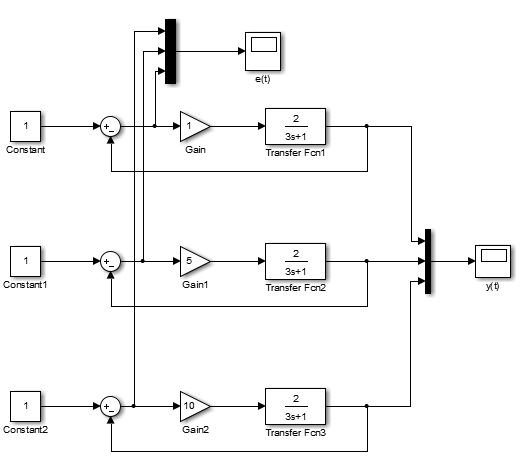
\includegraphics[width = 0.5\textwidth]{sxema1}
	\caption{Схема моделирования системы с астатизмом нулевого порядка}
\end{figure}
\begin{figure}[h!]
	\centering
	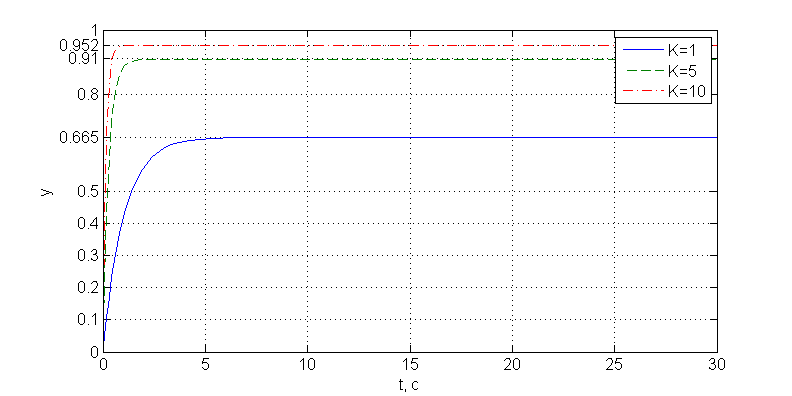
\includegraphics[width = 1\textwidth]{hinh2}
	\caption{Графики переходных процессов в стационарном режиме работы при различных K}
\end{figure}
\newpage
\begin{figure}[h!]
	\centering
	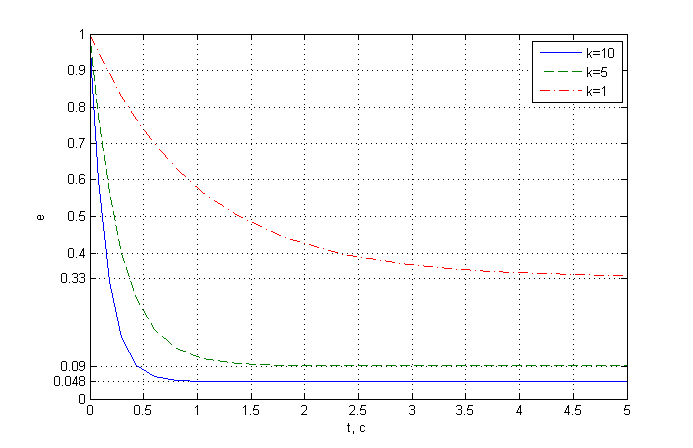
\includegraphics[width = 1\textwidth]{hinh1}
	\caption{Графики ошибки в системе в стационарном режиме при различных K}
\end{figure}
\hfill\\*
Аналитический расчет установивишихся значений ошибки:
\begin{equation}
\varepsilon=\frac{A}{1+k}
\end{equation}

\begin{align}
\varepsilon &=\frac{A}{1+k} =\frac{1}{1+2}=0.33 (K=1 ) \\
\varepsilon &=\frac{A}{1+k} =\frac{1}{1+10}=0.091 (K=5 ) \\
\varepsilon &=\frac{A}{1+k} =\frac{1}{1+20}=0.048 (K=10 )
\end{align}
\par
\paragraph{1.2 Исследование режима работы с постоянной скоростью: $g(t) = 0.5t$ }\hfill\par
На рисунке 4 представлена схема моделирования.На рисунке 5 представлен график переходного процесса при различнх K. На рисунке 6 - график ошибки при различных значениях K.
\begin{figure}[H]
	\centering
	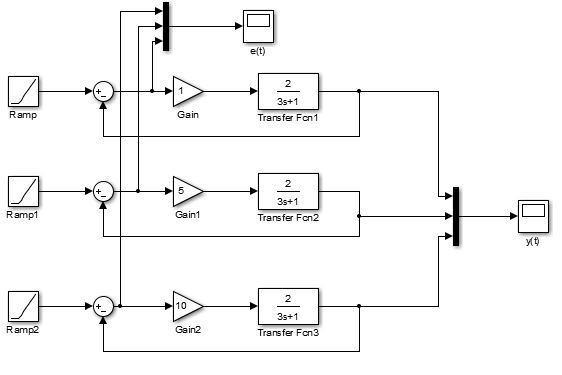
\includegraphics[width = 0.5\textwidth]{sxema2}
	\caption{Схема моделирования системы с астатизмом нулевого порядка}
\end{figure}
\begin{figure}[h]
	\centering
	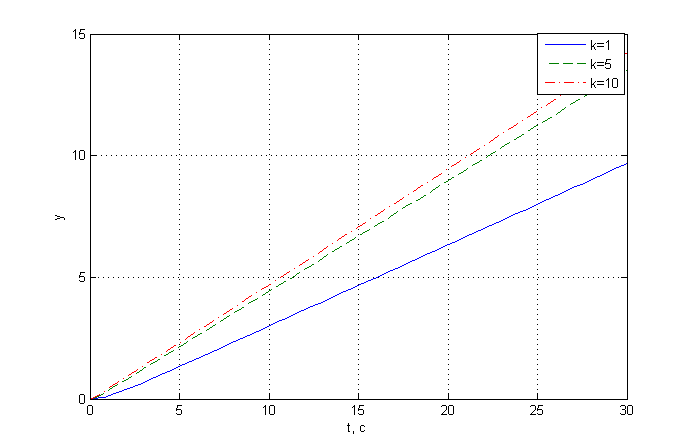
\includegraphics[width = 1\textwidth]{hinh4}
	\caption{Графики переходных процессов в режиме с постоянной скоростью при различных K}
\end{figure}
\begin{figure}[h]
	\centering
	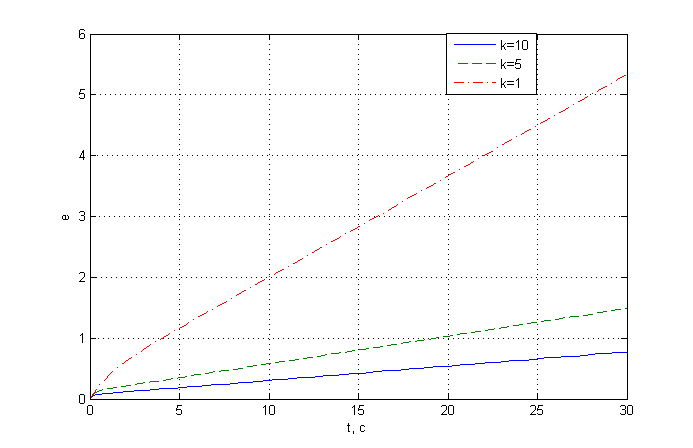
\includegraphics[width = 1\textwidth]{hinh3}
	\caption{Графики ошибки системы в режиме работы с постоянной скоростью  при различных K}
\end{figure}\hfill\\*
\newpage
\begin{flushleft}
	Аналитический расчет установивишихся значений ошибки:\\*
\end{flushleft} 
\begin{equation}
\varepsilon=\lim_{s \to 0} s(\frac{1}{1+W(s)})(\frac{V}{s^2})
\end{equation}
Во всех случаях $\varepsilon \to \infty$\\
\newpage
\begin{center}
	\section*{\centering 2 Исследование системы с астатизмом первого порядка}
\end{center}

\paragraph{2.1 Исследование стационарного режима работы: $g(t) = 1$}\hfill\par
На рисунке 7 представлена схема моделирования системы. На рисунках 8 и 9 - графики переходных процессов и ошибки при различных K, соответственно.
\begin{figure}[H]
	\centering
	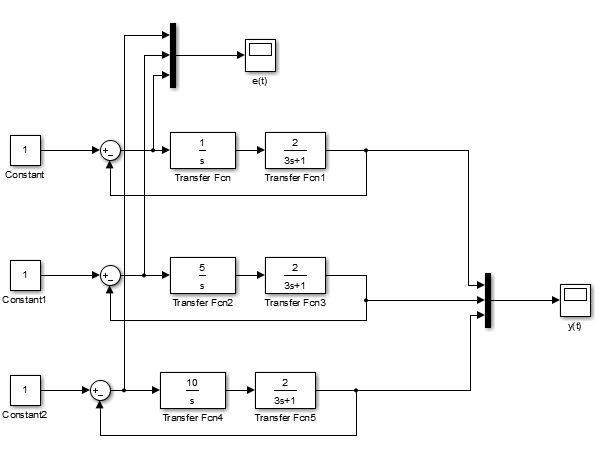
\includegraphics[width = 0.7\textwidth]{sxema3}
	\caption{Схема моделирования системы с астатизмом первого порядка}
\end{figure}
\hfill\\
\begin{figure}[h]
	\centering
	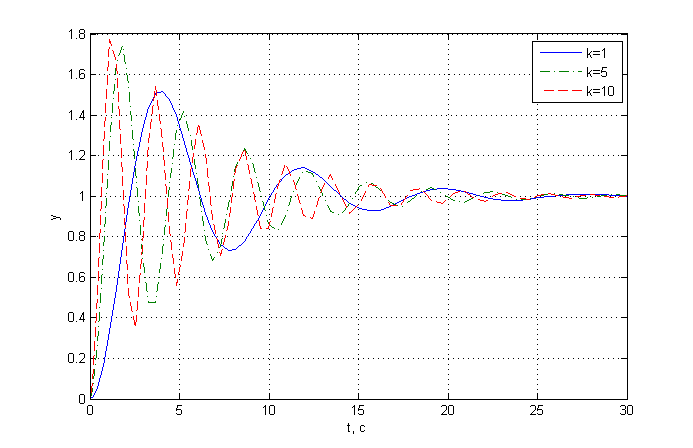
\includegraphics[width = 1\textwidth]{hinh5}
	\caption{Графики переходных процессов в стационарном режиме при различных K}
\end{figure}

\begin{figure}[h!]
	\centering
	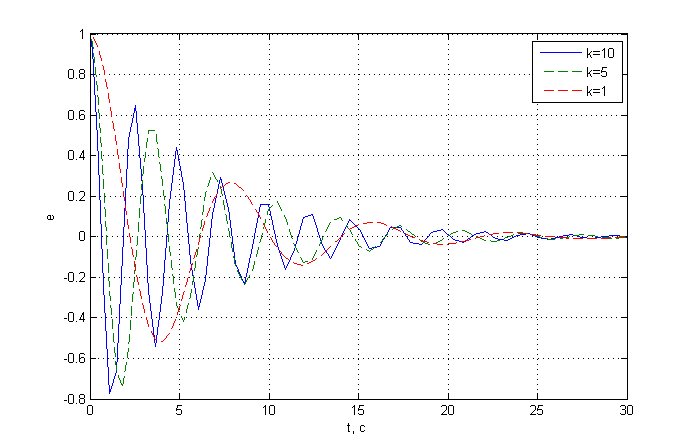
\includegraphics[width = 1\textwidth]{hinh6}
	\caption{Графики ошибки системы в стационарном режиме при различных K}
\end{figure}
\hfill\\*
\newpage
Аналитический расчет установивишихся значений ошибки:\\*
\begin{equation}
\varepsilon=\lim_{s \to 0} s(\frac{1}{1+W(s)})(\frac{A}{s})=\lim_{s \to 0} A(\frac{s}{s+k})=0
\end{equation}
\paragraph{2.2 Исследование режима движения с постоянной скростью: $g(t) = 0.5t$}\hfill\par
На рисунке 10 представлена схема моделирования.На рисунках 11 и 12 представлены графики переходных процессов и ошибки соответственно.
\begin{figure}[H]
	\centering
	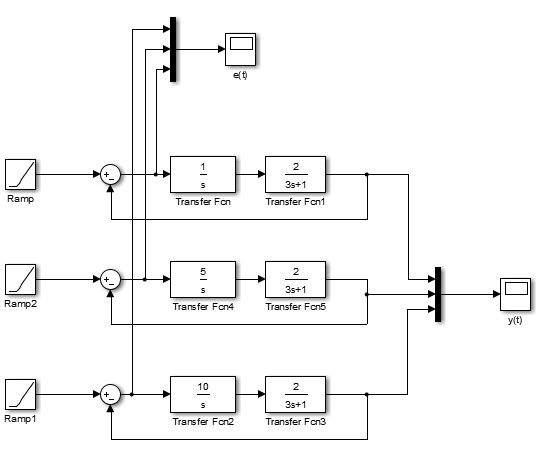
\includegraphics[width = 0.6\textwidth]{sxema4}
	\caption{Схема моделирования системы с астатизмом первого порядка}
\end{figure}
\begin{figure}[h]
	\centering
	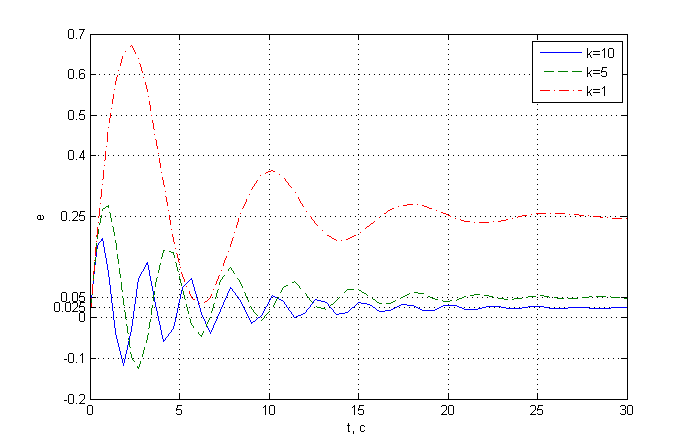
\includegraphics[width = 1\textwidth]{hinh8}
	\caption{Графики переходных процессов при движения с постоянной скоростью при различных K}
\end{figure}
\begin{figure}[H]
	\centering
	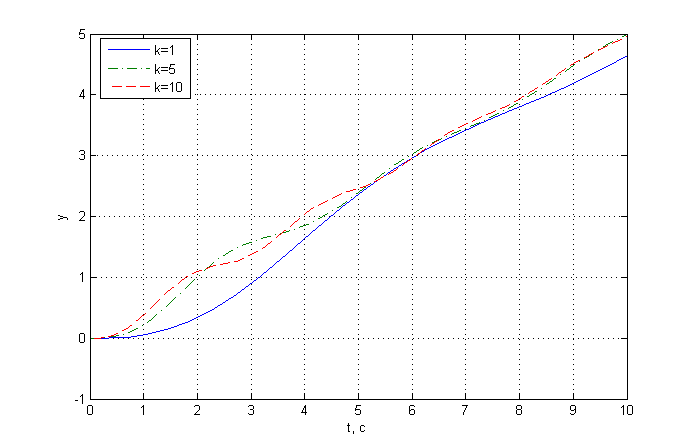
\includegraphics[width = 1\textwidth]{hinh7}
	\caption{Графики ошибки в режиме работы с постоянной скоростью при различных K}
\end{figure}\hfill\\*

Аналитическое подтверждение полученных результатов:\\*
\begin{equation}
\varepsilon=\lim_{s \to 0} s(\frac{1}{1+W(s)})(\frac{V}{s^2})
\end{equation}

\begin{align}
\varepsilon=\lim_{s \to 0} s(\frac{1}{1+W(s)})(\frac{V}{s^2})=\lim_{s \to 0} (\frac{V}{s})(\frac{s}{s+k})=0.5/2=0.25 (K=1) 
\end{align}
\begin{align}
\varepsilon=\lim_{s \to 0} s(\frac{1}{1+W(s)})(\frac{V}{s^2})=\lim_{s \to 0} (\frac{V}{s})(\frac{s}{s+k})=0.5/10=0.05(K=5) 
\end{align}
\begin{align}
\varepsilon=\lim_{s \to 0} s(\frac{1}{1+W(s)})(\frac{V}{s^2})=\lim_{s \to 0} (\frac{V}{s})(\frac{s}{s+k})=0.5/20=0.025(K=10)
\end{align}

\par

\paragraph{2.3 Исследование движения с постоянным ускорением: $g(t) = 0.25t^2$}\hfill\par
На рисунке 13 представлена схема моделирования.На рисунках 14 и 15 представлены графики переходных процессов и ошибки при движении с постоянным устокением.
\begin{figure}[h]
	\centering
	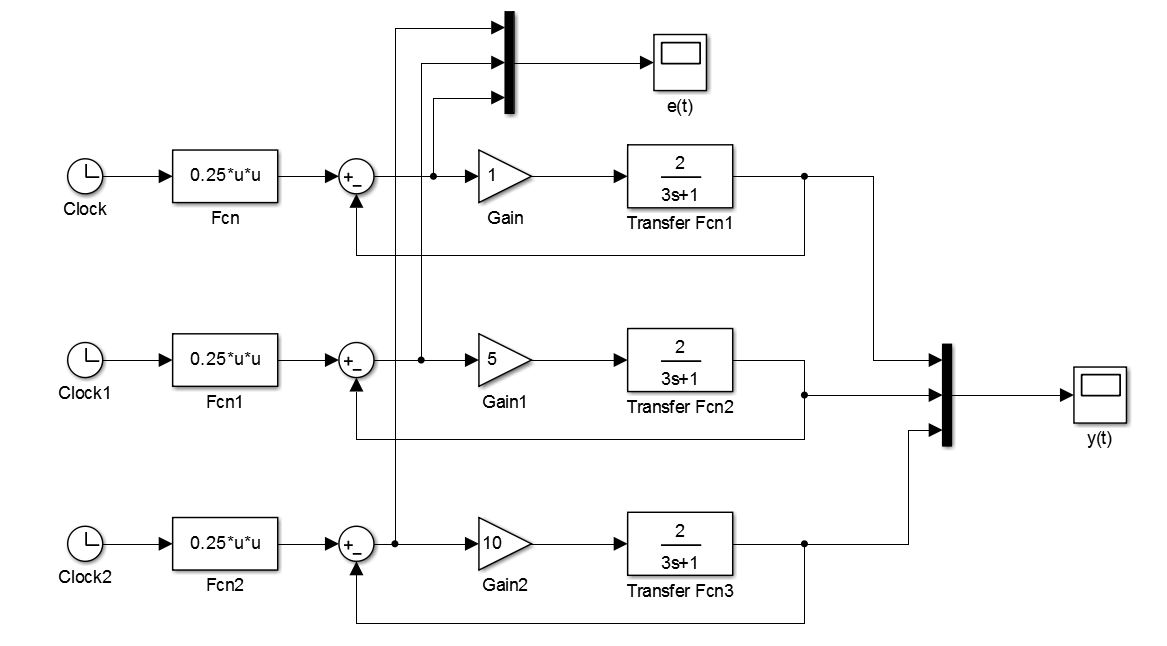
\includegraphics[width = 0.8\textwidth]{sxema5}
	\caption{Схема моделирования системы с астатизмом первого порядка}
\end{figure}

\begin{figure}[h!]
	\centering
	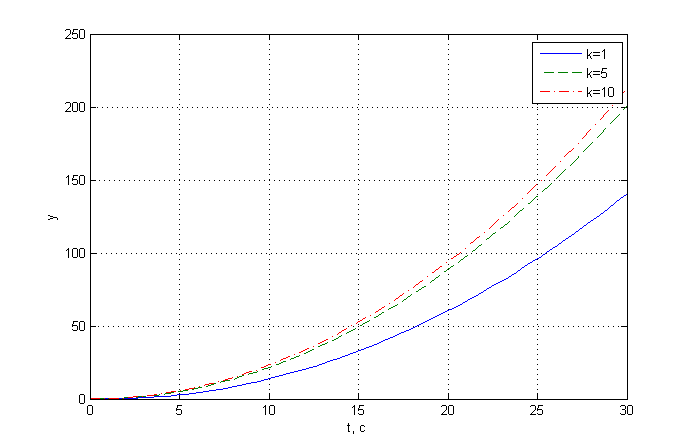
\includegraphics[width = 1\textwidth]{hinh10}
	\caption{Графики переходных процессов при движении с постоянным ускорением для различных К}
\end{figure}\hfill\\*
\newpage
\begin{figure}[h]
	\centering
	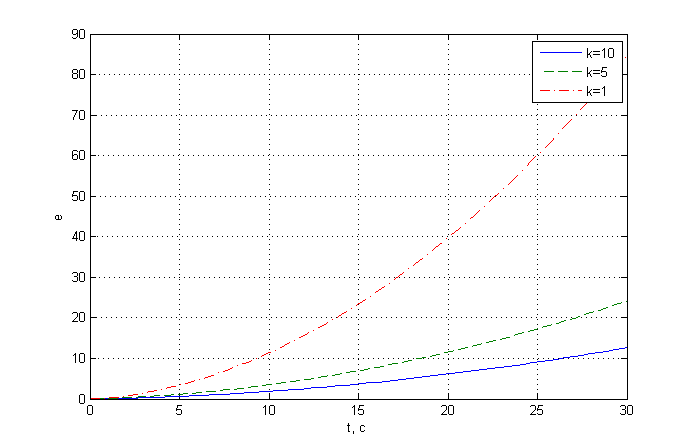
\includegraphics[width = 1\textwidth]{hinh9}
	\caption{Графики ошибки при движении с постоянным ускорением для различных К}
\end{figure}\hfill\\*
\newpage
\begin{center}
	\newpage
	\section*{\centering 3 Исследование влияния внешних возмущений}
\end{center}\par
На рисунке 16 представлена схема моделирования системы. На рисунка 17 и 18 - графики переходных процессов и ошибки для различных значений $f_1$ и $f_2$.\\*
\begin{figure}[h!]
	\centering
	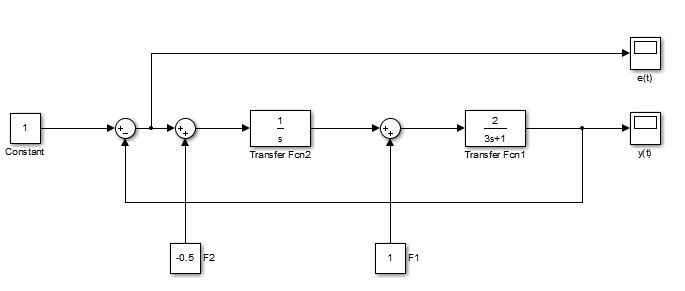
\includegraphics[width = 0.8\textwidth]{sxema6}
	\caption{Схема моделирования системы с внешними воздействиями}
\end{figure}
\begin{figure}[h!]
	\centering
	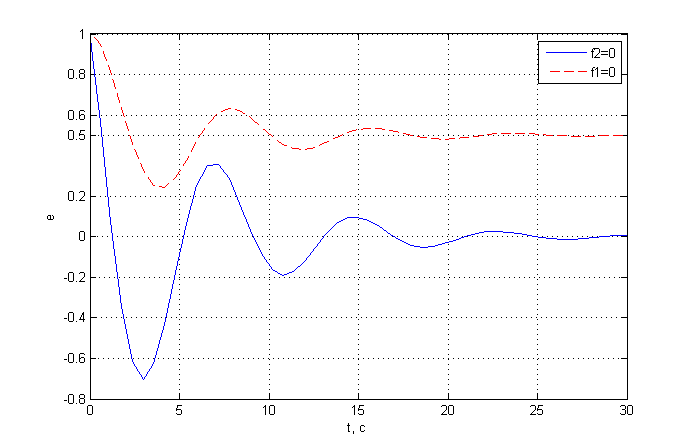
\includegraphics[width = 1\textwidth]{hinh11}
	\caption{Графики переходных процессов при различных значениях шумов}
\end{figure}
\newpage
\begin{figure}[h!]
	\centering
	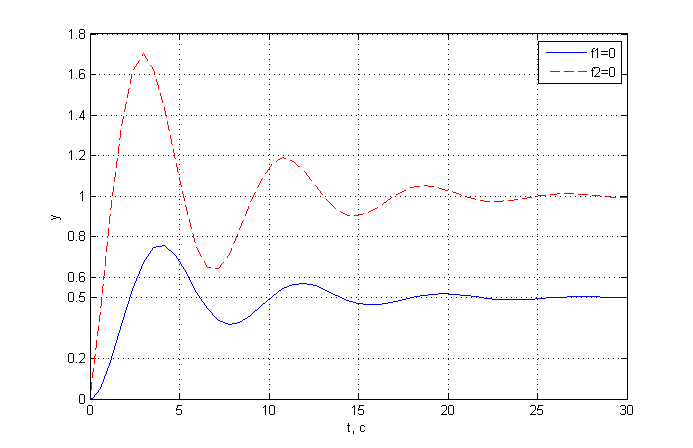
\includegraphics[width = 1\textwidth]{hinh12}
	\caption{Графики ошибки при различных значениях шумов}
\end{figure}\hfill\\*
Рассчитаем предельное значение установившейся ошибки: \\
\begin{align}
E=\frac{s}{W+s}G-\frac{sW}{W+s}F_{1}-\frac{W}{W+s}F_{2} 
\end{align}
Предельное значение установившейся ошибки $\varepsilon=0$ при $f_1$=1 и $f_2$=0 : \\
\begin{equation}
\varepsilon= \lim_{s\to 0}(\frac{s}{W+s}1-\frac{sW}{W+s}1-\frac{W}{W+s}0)=0
\end{equation}
Предельное значение установившейся ошибки $\varepsilon=0$ при $f_1$=0 и $f_2$=-0.5 : \\
\begin{equation}
\varepsilon= \lim_{s\to 0}(\frac{s}{W+s}1-\frac{sW}{W+s}0-\frac{W}{W+s}(-0.5))=\lim_{s\to 0}0.5\frac{2}{3s^2+s+2}=0.5
\end{equation}
\newpage 
\begin{center}
	\section*{\centering 4 Исследование установившейся ошибки при произвольном входном воздействии}
\end{center}\par
На рисунке 19 предствалена схема моделирования системы. На рисунке 20 график переходного процесса при произвольном входном воздействии $2+3\sin(0.5t)$.
\begin{figure}[h!]
	\centering
	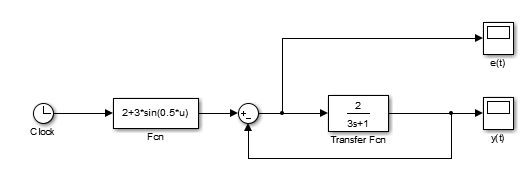
\includegraphics[width = 0.8\textwidth]{sxema7}
	\caption{Схема моделирования системы с произвольным входным воздействием}
\end{figure}
\begin{figure}[h!]
	\centering
	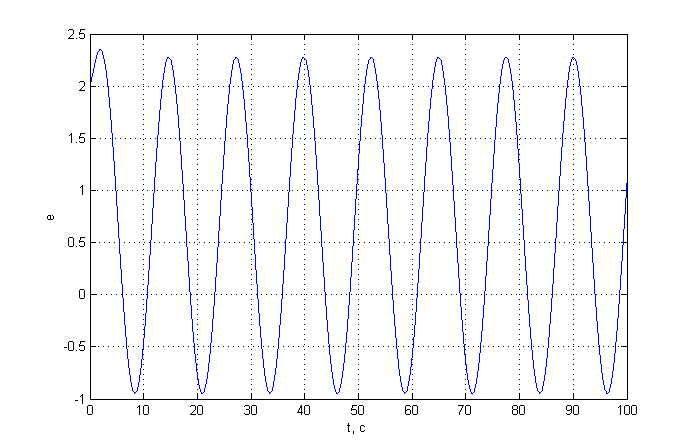
\includegraphics[width = 1\textwidth]{hinh13}
	\caption{График переходного процесса при произвольном входном воздействии} 
\end{figure}
\hfill\\*
Ошибка рассчитывается по формуле:
\begin{equation}
e(t)=c_0g(t)+c_1\frac{d}{dt}g(t)+c_2\frac{d^2}{2!dt^2}g(t)
\end{equation}
Где \\
	
\begin{align}
\Phi=\frac{1}{1+W(s)}
\end{align}
\begin{align}
c0=Ф(s)|_{s=0}=0.33
\end{align}
\begin{align}
c1=\frac{d\Phi(s)}{ds} |_{s=0}=0.66
\end{align}
\begin{align}
c2=\frac{d^2\Phi(s)}{ds^2} |_{s=0}=-1.33 
\end{align}
В итоге:
\begin{equation}
 e(t)=0.66+1.495\sin(0.5t)+0.99\cos(0.5t)
 \end{equation}
\newline
На рисунке 21 сопоставляется рассчитанная ошибка и ошибка полученая моделированием.
\begin{figure}[h!]
	\centering
	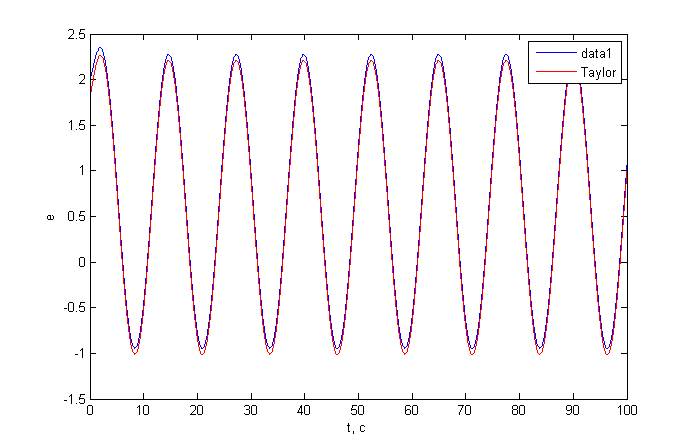
\includegraphics[width = 1\textwidth]{hinh14}
	\caption{Графики ошибок полученных аналитически и моделированием} 
\end{figure}

\newpage

	\section*{\centering Выводы}
 В данной работе мы исследовали системы с разными порядками астатизма и различными входными и возмущающими воздействиями. В частности, системы с астатизмом первого порядка нечувствительны к постоянным возмущениям.При исследовании стационарного режима работы, убедились в том, что при g = A, и увеличении коэффициента усиления k ошибка стремиться к нулю. 
 Убедились в том, что при увеличении прядка астатизма, ошибка, при статическом входном возвдействии ошибка равна нулю.
 Внешние возмущения могут оказвать довольно сильное влияние - изменение выходного сигнала в 2 раза, сильное перерегулироване.
\end{document}